	
In these experiments, several current techniques (2D Feature Matching (FM-2D), 3D Feature Matching (FM-3D), ICP and PCA) are compared to the FVR technique in terms of stereo camera registration accuracy. To this end, five datasets from the Kitti Vision Benchmark dataset \cite{Geiger13Vision} were used. Each data set scene is a complicated outdoor environment filmed using an autonomous driving platform. A majority of frames contain moving objects which interfere with the registration process of several algorithms. \\

Each Kitti Vision Benchmark Data Set contains accurate laser scans, stereo gray-scale images, stereo rgb-images and GPS and IMU data. In order to simulate the theoretical situation in which stereo cameras generate the most accurate depth maps, the laser scans are used in place of depth data computed by a stereo disparity algorithm. Therefore, in these experiments, only the laser scans and stereo color and gray-scale images are used. \\

%keep
\begin{figure*}[t]
\centering
\begin{subfigure}[b]{1.5in}
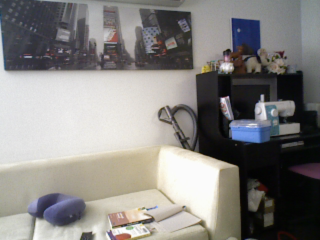
\includegraphics[width=1.5in]{{images/experiments/test_data/Apartment.Texture.rotate.0}.png}
\caption{Frame 1}
\end{subfigure}%
\begin{subfigure}[b]{1.5in}
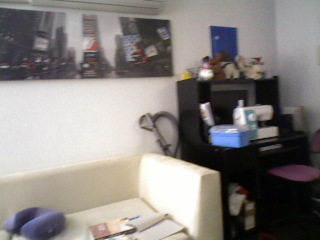
\includegraphics[width=1.5in]{{images/experiments/test_data/Apartment.Texture.rotate.1}.png}
\caption{Frame 10}
\end{subfigure}%
\begin{subfigure}[b]{1.5in}
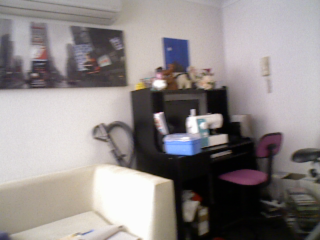
\includegraphics[width=1.5in]{{images/experiments/test_data/Apartment.Texture.rotate.2}.png}
\caption{Frame 15}
\end{subfigure}%
\begin{subfigure}[b]{1.5in}
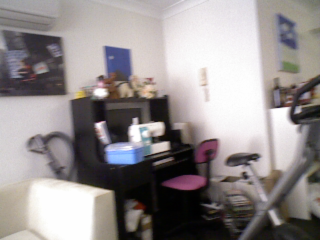
\includegraphics[width=1.5in]{{images/experiments/test_data/Apartment.Texture.rotate.3}.png}
\caption{Frame 20}
\end{subfigure}%
\caption{Apartment.Texture.rotate Scene.}
\label{fig:Apartment_Texture_rotate}
\end{figure*}




The five stereo data-sets used in the experiments are shown in figures \ref{fig:KT1DSS}, \ref{fig:KT2DSS}, \ref{fig:KT5DSS}, \ref{fig:KT91DSS} and \ref{fig:KT95DSS}. The first scene is the Kitti 0001 Sync Data Set, this scene has 107 frames. This data set contains 12 cars, 2 cyclists and a tram. The tram and cyclists are non static objects within the scene, making it more difficult for the current set of reconstruction algorithms which rely on scenes being primarily static in nature. To the right in this dataset, there is a tram-line and some trees and gardens, to the left is a residential street. The second scene is the Kitti 0002 Sync Data Set, this set is 76 frames long. It contains 1 car and two cyclists which are non-static objects. Within this scene there is a long brick wall hiding some tall trees, several cyclists ride along next to the wall. To the left, there are are some grassy areas, some buildings and some parked cars. \\

At 153 frames, the Kitti 0005 Sync Data Set is also used. This scene contains 9 cars, 3 vans, 2 pedestrians and 1 cyclist. Because of the size of the van and the other non-static objects within the scene, this appears to be one of the more difficult scenes to register. The camera winds through several different streets as opposed to the previous data sets which are mostly of one long road. The fourth dataset used, the Kitti 0091 Sync Data Set is composed of 339 frames making it the largest data set used in these experiments. This data set contains 2 cars, a van, 42 pedestrians, 14 sitters, 8 cyclists and 1 miscellaneous object. Due to containing so many non-static objects this scene is also considered difficult like the Kitti 0005 Data Set. \\

The last Kitti Vision Benchmark Data Set used is the Kitti 0095 Data Set. Unlike the previous data sets, all 267 frames only contain static object, and the scenes are made up primarily of small winding streets. \\ 

Experiments are tabled in full at per frame intervals in the appendix (Appendix \ref{StereoResultsRaw}). Here, registration errors are presented where frame $n$ is registered against frame $n+1$ and the registration error is reported for each algorithm. The error function used is the Mean Squared Error $MSE(P,Q)$. This error is computed between the consecutive frames after registration. This error value is computed as in equation \ref{eqn:msesota}. Here, the function $Register(x)$ is replaced by the registration method being tested. \\

\begin{equation} \label{eqn:msesota}
Error(frame_1, frame_2) =  \frac{Register(frame_1), frame2}{MSE(frame_1,frame_2)}
\end{equation}

\begin{figure*}[t]
\centering
\begin{subfigure}[b]{1.5in}
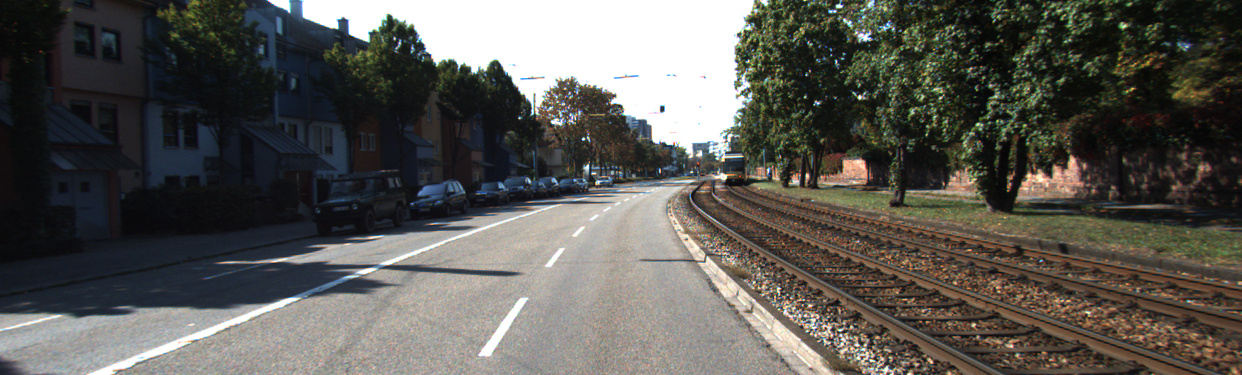
\includegraphics[width=1.5in]{{images/experiments/stereo/1.1}.png}
\caption{Frame 1}
\end{subfigure}%
\begin{subfigure}[b]{1.5in}
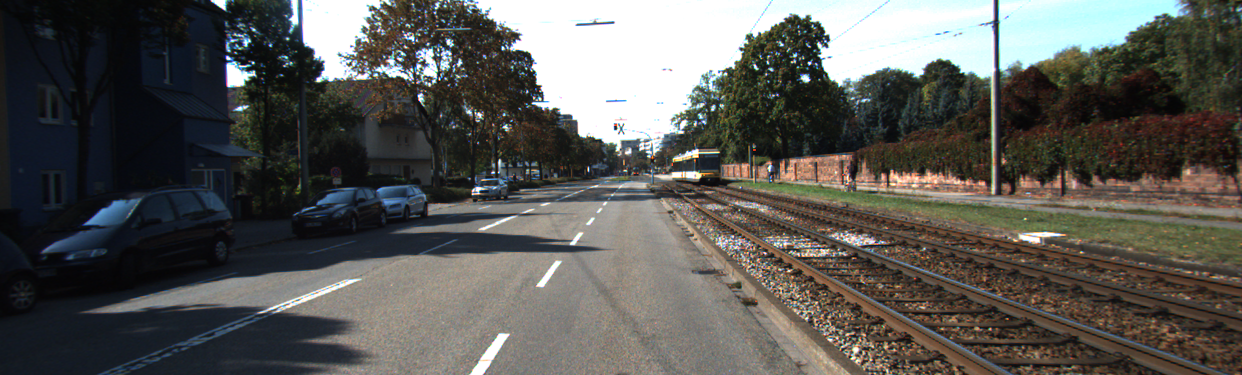
\includegraphics[width=1.5in]{{images/experiments/stereo/1.2}.png}
\caption{Frame 39}
\end{subfigure}%
\begin{subfigure}[b]{1.5in}
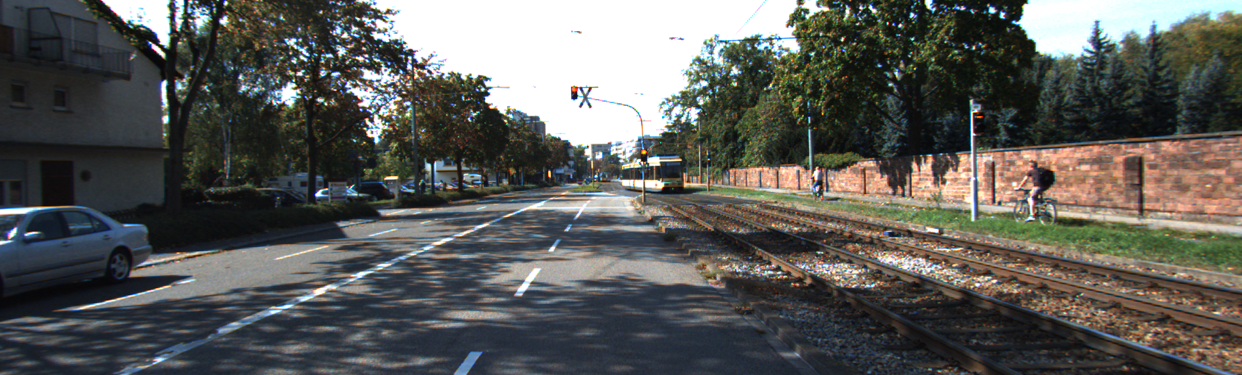
\includegraphics[width=1.5in]{{images/experiments/stereo/1.3}.png}
\caption{Frame 77}
\end{subfigure}%
\begin{subfigure}[b]{1.5in}
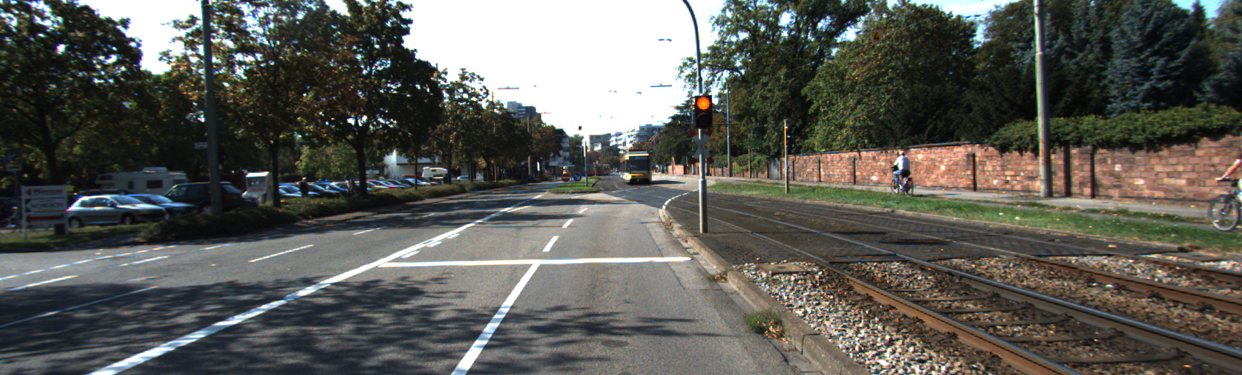
\includegraphics[width=1.5in]{{images/experiments/stereo/1.4}.png}
\caption{Frame 114}
\end{subfigure}%
\caption{Kitti 0001 Sync Data Set Sample}
\label{fig:KT1DSS}
\end{figure*}



%% sync 0001

\begin{figure}
\centering
\begin{tabular}{ccc}
\hline
\textbf{Algorithm} & \textbf{Median Error $\times$ 1000} & \textbf{\% best results}\\ \hline
FM2D	& 5.28 & 13.21\%\\
FM3D	& 9235.71 & 0.94\%\\
ICP	& 5.15 & 27.36\%\\
PCA	& 5.66 & 2.83\%\\
FVR	& 5.5 & 13.21\%\\
FFVR	& 5.59 & 7.55\%\\
FVR3D	& 5.1 & 34.91\%\\
\end{tabular}
\caption{Statistics for the Kitti Data 0001 Sync Data Set}
\label{tab:kittidata0001sync}
\end{figure} 

The summary of these results is also tabled here for convenience. For each algorithm, the median registration error is provided. This is computed by listing and sorting the registration error values for a particular algorithm and selecting the value in the middle. Assisting this is the percent of best results metric. This measures in percentage, the frequency of times a particular algorithm achieved the best (lowest error) registration result compared to the other algorithms tested. An algorithm with a lower median error compared to another algorithm would be said to have performed better overall. Additionally, if an algorithm has a higher percentage of best results, it outperformed the other algorithms a majority of the time. If an algorithm achieved an average percentage of bests results but a higher median error, this could be explained by outliers. If an algorithm achieved a lower median error but did not achieve the highest percentage of best results, it may be due to having a very competitive and consistent registration error. \\

Table \ref{tab:kittidata0001sync} presents results for the Kitti 0001 Sync Data Set, some example color frames are shown in figure \ref{fig:KT1DSS}. The road in which this scene was filmed contains a tram-line and moving tram as well as a garden area to the right and a line of parked cars and houses under cover of shadows to the left. Registration statistics were taken over the full length of this data set, which is 107 frames for the Kitti 0001 Sync Data Set. Results show that FVR3D achieved the lowest median registration error, ICP achieved the next lowest followed by FM2D and the FVR method. FVR3D also achieved the highest percentage of best best frame registration results at ~34.91\% compared to runner-up ICP's ~27.36\%. If the FVR methods were combined as a single hybrid method, they would have computed the best registration result 55.67\% of the time. The FVR method alone outperformed FFVR, PCA and FM3D. The FM3D method (which had several frame registration failures, as is evident in its statistics) and the PCA method were the worse performers on this dataset. It can be seen that the FFVR, whilst faster than the FVR method is slightly worse off in terms of performance. \\ 


%% sync 0002
\begin{figure}
\centering
\begin{tabular}{ccc}
\hline
\textbf{Algorithm} & \textbf{Median Error $\times$ 1000} & \textbf{\% best results}\\ \hline
FM2D	& 4.78 & 5.33\%\\
FM3D	& 4.85 & 6.67\%\\
ICP	& 4.43 & 30.67\%\\
PCA	& 4.86 & 6.67\%\\
FVR	& 4.67 & 6.67\%\\
FFVR	& 5.23 & 5.33\%\\
FVR3D	& 4.27 & 38.67\%\\
\end{tabular}
\caption{Statistics for the Kitti Data 0002 Sync Data Set}
\label{tab:kittidata0002sync}
\end{figure} 



\begin{figure*}[t]
\centering
\begin{subfigure}[b]{1.5in}
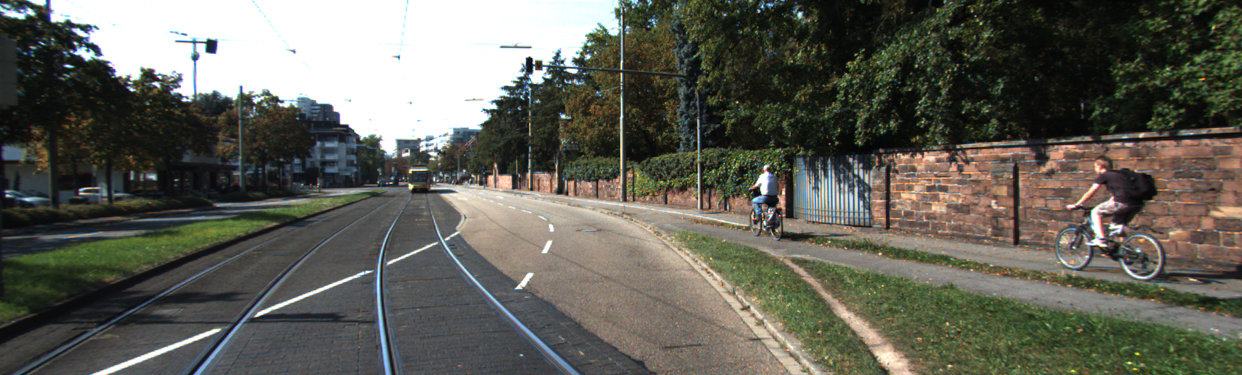
\includegraphics[width=1.5in]{{images/experiments/stereo/2.1}.png}
\caption{Frame 1}
\end{subfigure}%
\begin{subfigure}[b]{1.5in}
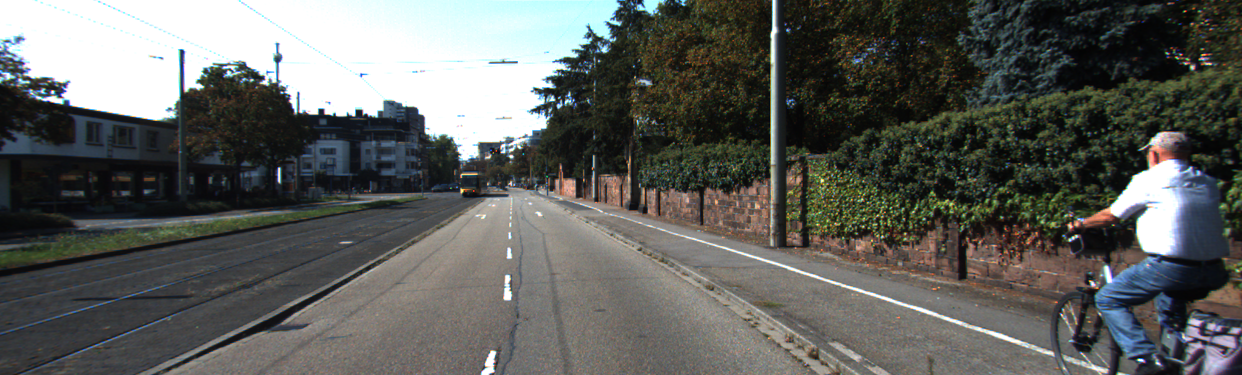
\includegraphics[width=1.5in]{{images/experiments/stereo/2.2}.png}
\caption{Frame 28}
\end{subfigure}%
\begin{subfigure}[b]{1.5in}
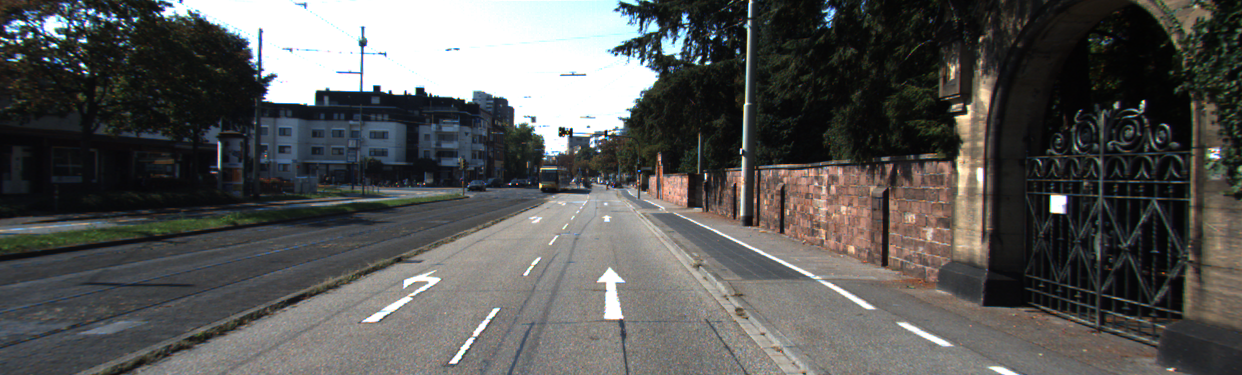
\includegraphics[width=1.5in]{{images/experiments/stereo/2.3}.png}
\caption{Frame 56}
\end{subfigure}%
\begin{subfigure}[b]{1.5in}
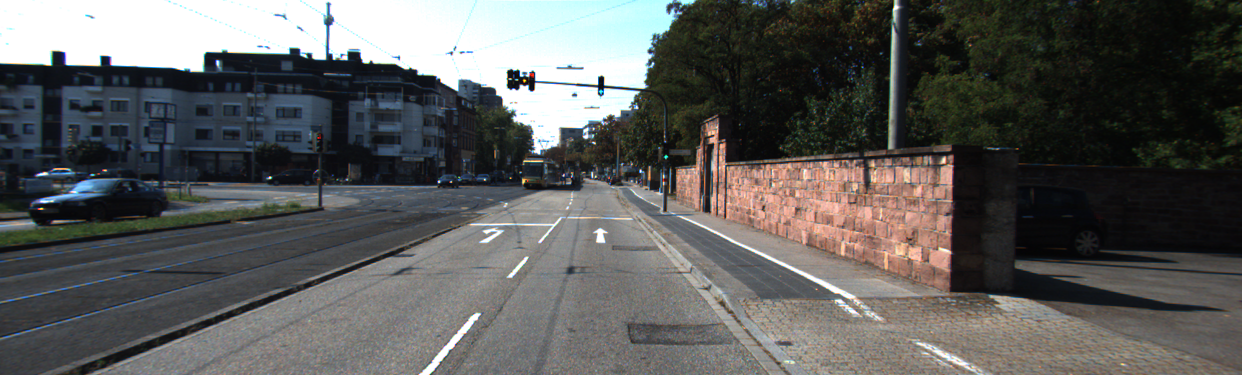
\includegraphics[width=1.5in]{{images/experiments/stereo/2.4}.png}
\caption{Frame 83}
\end{subfigure}%
\caption{Kitti 0002 Sync Data Set Sample}
\label{fig:KT2DSS}
\end{figure*}


Table \ref{tab:kittidata0002sync} presents median error and \% best result statistics for the Kitti 0002 Sync Data Set, example color frames are shown in figure \ref{fig:KT2DSS}. The road in which this scene contains some parked cars to the left as well as a building, some grass and some large trees. To the right there is an orange brick wall and some trees and gardens as well as two moving cyclists. Results for the full 74 frames of the data set show that the FVR3D method achieved the lowest median registration error at 4.27. The ICP algorithm achieved the next best result at 4.43 and the non-rotation-invariant FVR method achieved the 3rd best result. Combined, the FVR based methods achieved the best result ~50.67\% of the time compared to ICP's 30.67\%. On this scene, the FM3D method did not have as many registration failures and achieved a better result compared to the FFVR method and a result which was fairly even with the PCA method. \\ 



%% 0005
\begin{figure}
\centering
\begin{tabular}{ccc}
\hline
\textbf{Algorithm} & \textbf{Median Error $\times$ 1000} & \textbf{\% best results}\\ \hline
FM2D	& 3.39 & 39.22\%\\
FM3D	& 3.83 & 0\%\\
ICP	& 3.49 & 25.49\%\\
PCA	& 4.06 & 0\%\\
FVR	& 3.7 & 5.88\%\\
FFVR	& 4.25 & 1.96\%\\
FVR3D	& 3.42 & 27.45\%\\
\end{tabular}
\caption{Statistics for the Kitti Data 0005 Sync Data Set}
\label{tab:kittidata0005sync}
\end{figure} 

Statistics for the Kitti 0005 Sync Data Set are presented in table \ref{tab:kittidata0005sync}. The scene captured in this dataset was more difficult than previous scenes as it contains 2 moving cyclists and 1 large van which are both moving around in the scene without any relation to camera movement. In other words, these non-static objects cause major difficulties in most registration algorithms. In the full 152 frames of the dataset, FM2D performed best with the lowest median error and highest percentage of best results. Next, FVR3D also performed well with the second best median error and percentage of best results measurement. ICP came third best achieving the third best median error and percentage of best results. In the results for this dataset, FVR outperformed the FFVR method, as well as PCA and FM3D. Combined, the FVR algorithms achieved the best registration result 35.29\% of the time, which is still below the performance of FM2D on this dataset. \\

\begin{figure*}[t]
\centering
\begin{subfigure}[b]{1.5in}
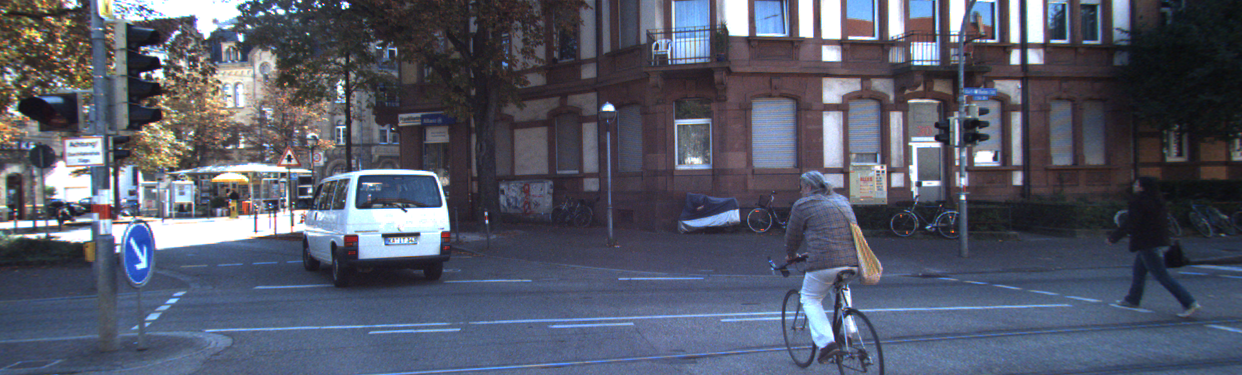
\includegraphics[width=1.5in]{{images/experiments/stereo/5.1}.png}
\caption{Frame 1}
\end{subfigure}%
\begin{subfigure}[b]{1.5in}
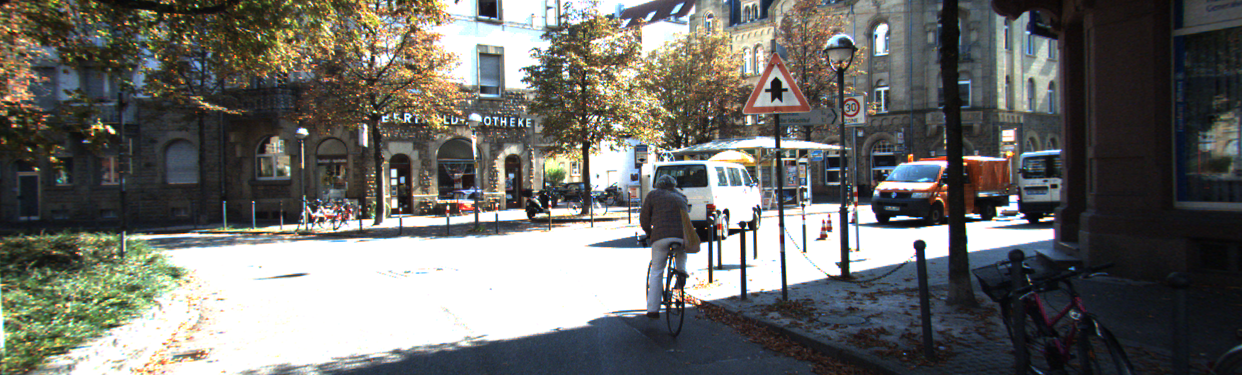
\includegraphics[width=1.5in]{{images/experiments/stereo/5.2}.png}
\caption{Frame 54}
\end{subfigure}%
\begin{subfigure}[b]{1.5in}
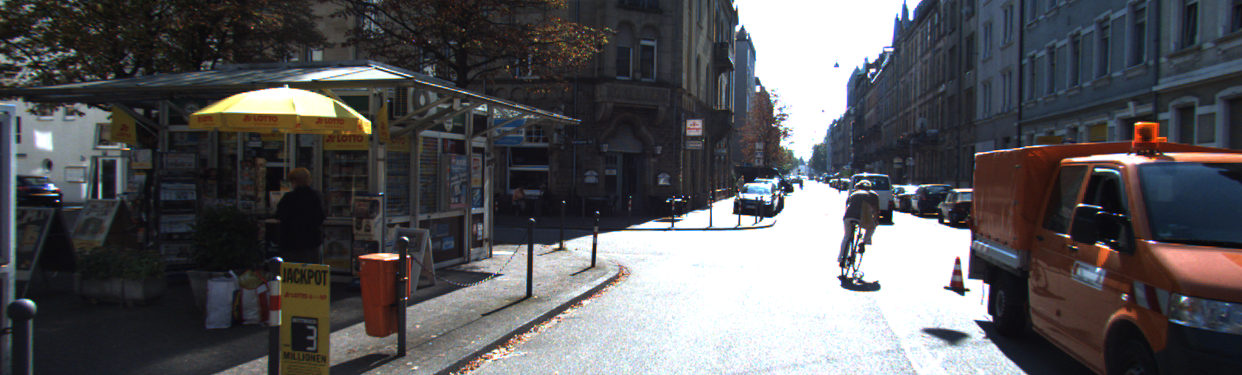
\includegraphics[width=1.5in]{{images/experiments/stereo/5.3}.png}
\caption{Frame 107}
\end{subfigure}%
\begin{subfigure}[b]{1.5in}
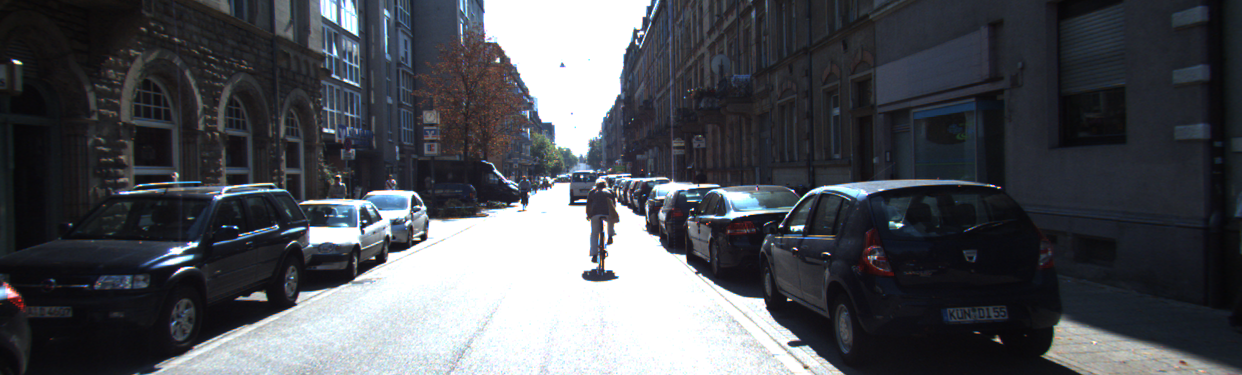
\includegraphics[width=1.5in]{{images/experiments/stereo/5.4}.png}
\caption{Frame 160}
\end{subfigure}%
\caption{Kitti 0005 Sync Data Set Sample}
\label{fig:KT5DSS}
\end{figure*}


%% kitti dataset 0091 Sync

\begin{figure}
\centering
\begin{tabular}{ccc}
\hline
\textbf{Algorithm} & \textbf{Median Error $\times$ 1000} & \textbf{\% best results}\\ \hline
FM2D	& 3.6 & 25.96\%\\
FM3D	& 4.04 & 1.18\%\\
ICP	& 3.61 & 23.6\%\\
PCA	& 4.1 & 1.77\%\\
FVR	& 3.93 & 12.09\%\\
FFVR	& 3.78 & 10.03\%\\
FVR3D	& 3.6 & 25.37\%\\
\end{tabular}
\caption{Statistics for the Kitti Data 0091 Sync Data Set}
\label{tab:kittidata0091sync}
\end{figure} 

Table \ref{tab:kittidata0091sync} presents results for the Kitti 0091 Data Set. This is the largest data set tested at 338 frames. The scene filmed in this dataset is that of an outdoors inner city. It contains many moving agents making it a scene which is difficult to register for most registrations algorithms. Specifically, it contains two cars, a van, 42 pedestrians and 8 cyclists. Registration results show FVR3D and FM2D achieved the best median error result with ICP achieving a close third place. In terms of this metric, FFVR outperforms FVR and they both outperform PCA and FM3D. Regarding the percentage of best results metric, FM2D achieved the highest percentage with ~\%25.96. FVR3D achieved the second best result at ~25.37\%. The FVR based methods performed well on this dataset, a hybrid approach would have achieved the best results 47.49\% of the time.  \\  	


\begin{figure*}[t]
\centering
\begin{subfigure}[b]{1.5in}
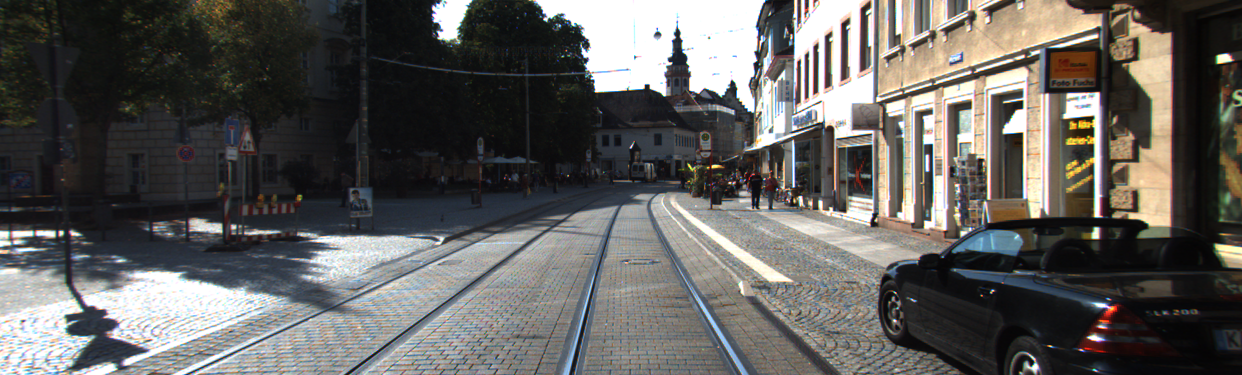
\includegraphics[width=1.5in]{{images/experiments/stereo/91.1}.png}
\caption{Frame 1}
\end{subfigure}%
\begin{subfigure}[b]{1.5in}
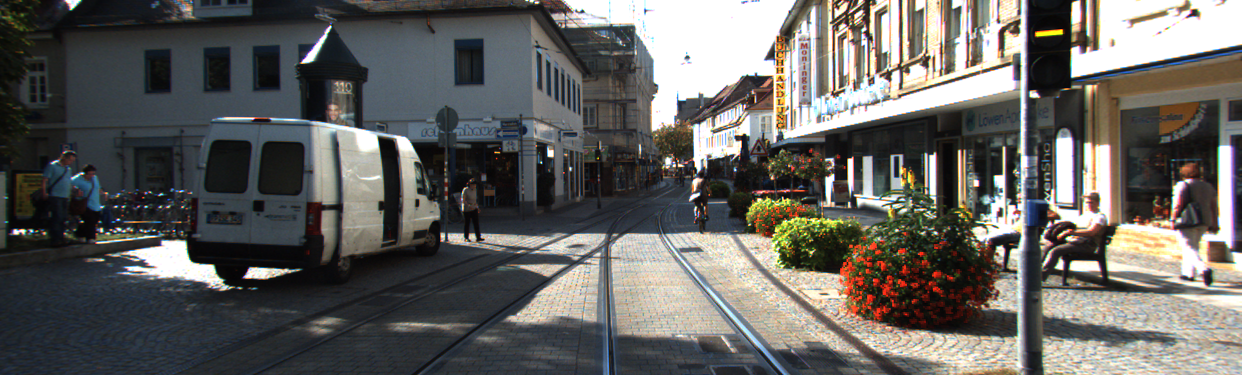
\includegraphics[width=1.5in]{{images/experiments/stereo/91.2}.png}
\caption{Frame 116}
\end{subfigure}%
\begin{subfigure}[b]{1.5in}
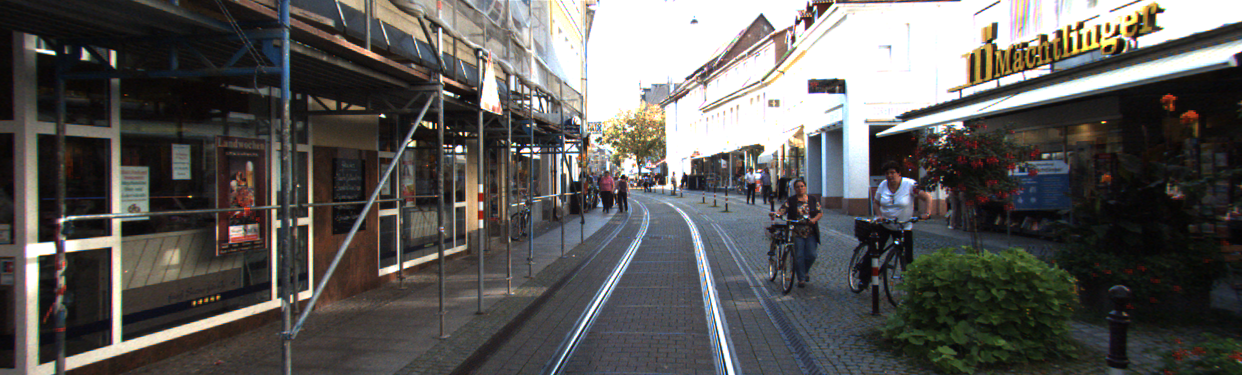
\includegraphics[width=1.5in]{{images/experiments/stereo/91.3}.png}
\caption{Frame 231}
\end{subfigure}%
\begin{subfigure}[b]{1.5in}
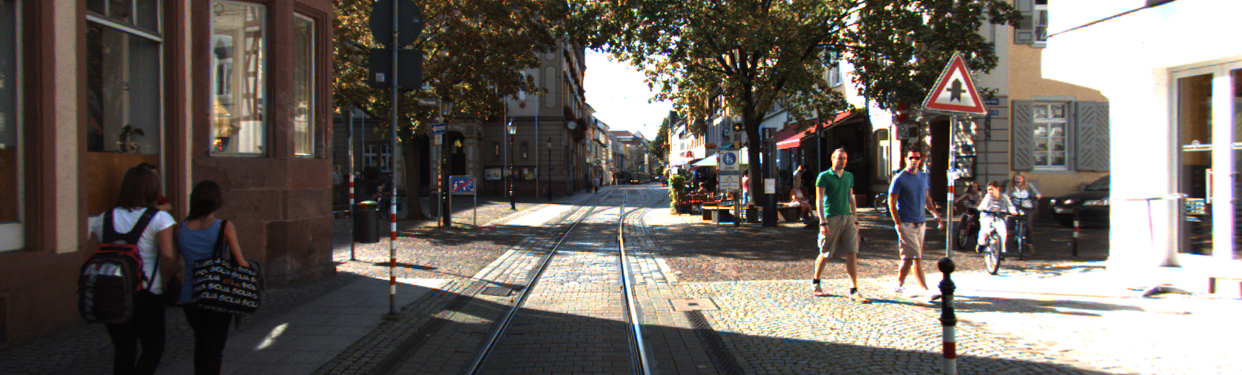
\includegraphics[width=1.5in]{{images/experiments/stereo/91.4}.png}
\caption{Frame 346}
\end{subfigure}%
\caption{Kitti 0091 Sync Data Set Sample}
\label{fig:KT91DSS}
\end{figure*}


%% sync 0095

\begin{figure}
\centering
\begin{tabular}{ccc}
\hline
\textbf{Algorithm} & \textbf{Median Error $\times$ 1000} & \textbf{\% best results}\\ \hline
FM2D	& 4.19 & 16.48\%\\
FM3D	& 5.18 & 0\%\\
ICP	& 4.4 & 22.85\%\\
PCA	& 5.32 & 0.37\%\\
FVR	& 4.68 & 17.23\%\\
FFVR	& 4.73 & 5.62\%\\
FVR3D	& 4.13 & 37.45\%\\
\end{tabular}
\caption{Statistics for the Kitti Data 0095 Sync Data Set}
\label{tab:kittidata0095sync}
\end{figure} 

Results for the Kitti 00095 Data Set are presented in table \ref{tab:kittidata0095sync}. This scene was much more static than the previous scenes. It contains primarily parked cars and buildings in an inner city environment. There are a few pedestrians and cyclists which are moving agents within the scene. This dataset is 266 frames and results show that FVR3D achieves both the best (lowest) median error score and the highest percentage of best results score at ~37.45\%. The FVR based methods have a hybrid percentage of best results value of 60.3\%. ICP achieved the seconds highest percentage of best results and FM2D achieved the 3rd best result. \\  



\begin{figure*}[t]
\centering
\begin{subfigure}[b]{1.5in}
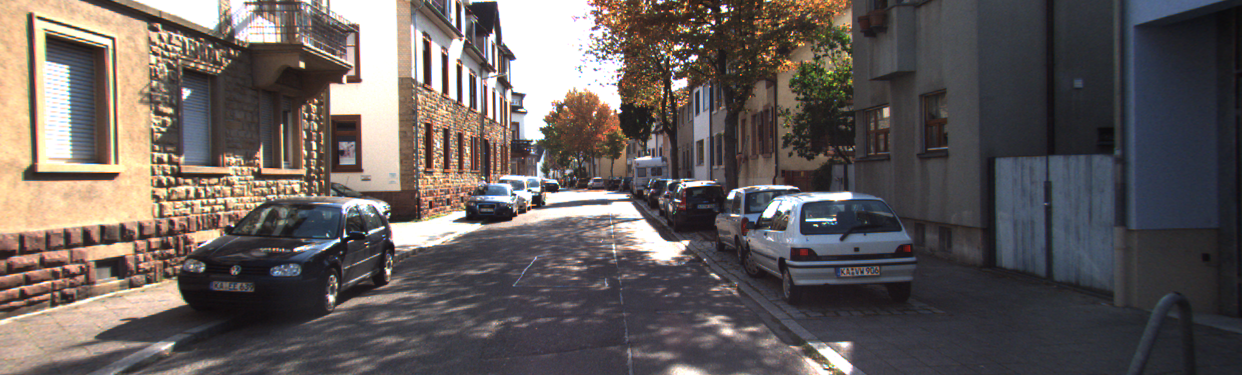
\includegraphics[width=1.5in]{{images/experiments/stereo/95.1}.png}
\caption{Frame 1}
\end{subfigure}%
\begin{subfigure}[b]{1.5in}
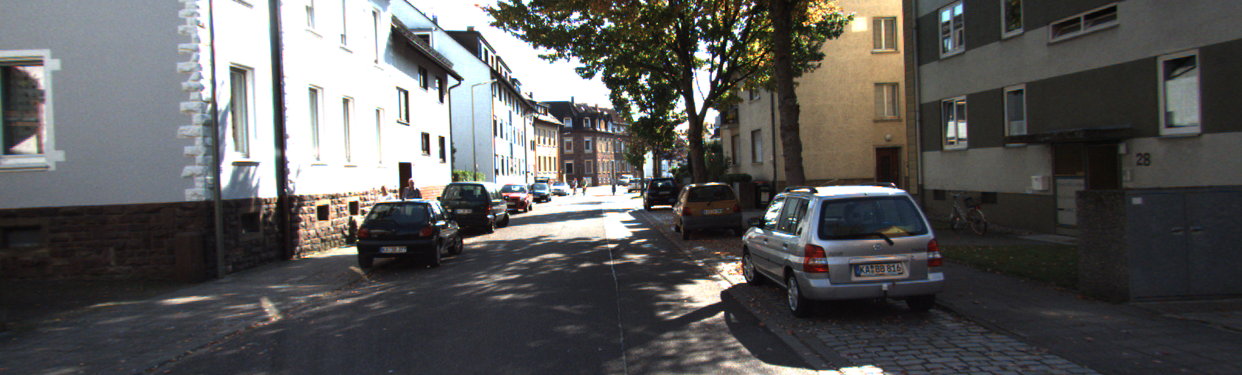
\includegraphics[width=1.5in]{{images/experiments/stereo/95.2}.png}
\caption{Frame 92}
\end{subfigure}%
\begin{subfigure}[b]{1.5in}
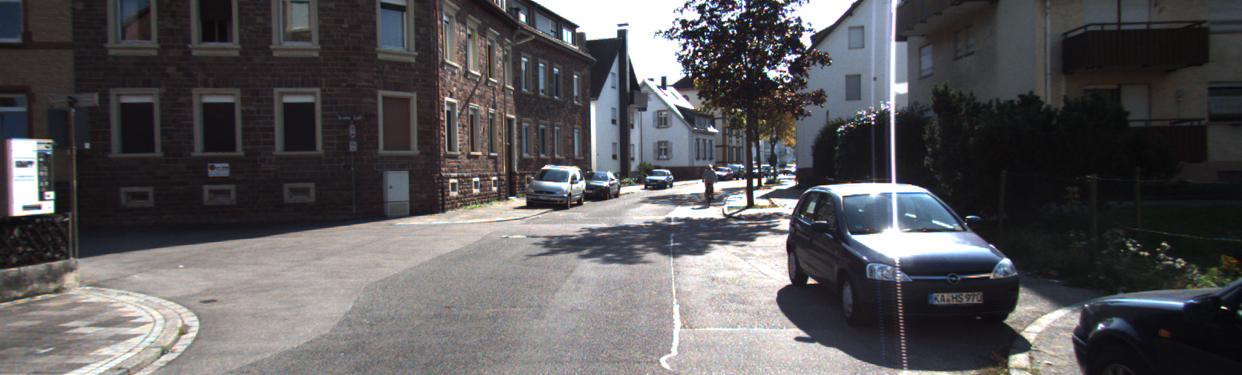
\includegraphics[width=1.5in]{{images/experiments/stereo/95.3}.png}
\caption{Frame 183}
\end{subfigure}%
\begin{subfigure}[b]{1.5in}
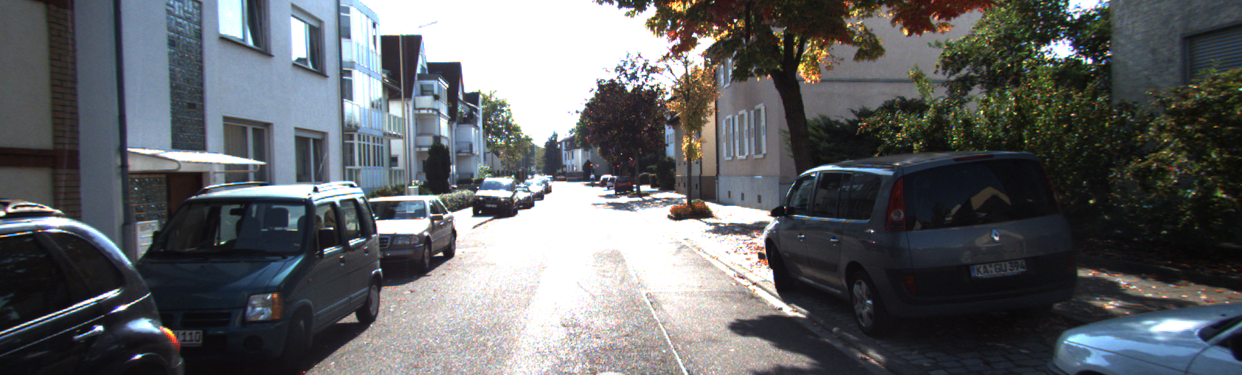
\includegraphics[width=1.5in]{{images/experiments/stereo/95.4}.png}
\caption{Frame 274}
\end{subfigure}%
\caption{Kitti 0095 Sync Data Set Sample}
\label{fig:KT95DSS}
\end{figure*}
